%%%%%%%%%%%%%%%%%%%%%%%%%%%%%%%%%%%%%%%%%%%%%%%%%%%%%%%%%%%%%%%%%%%%%%%%%%%%%%%%%%%%%%%%%%%%%
%%									Chapitre Approche de partitionnement et de distribution des graphes
%%%%%%%%%%%%%%%%%%%%%%%%%%%%%%%%%%%%%%%%%%%%%%%%%%%%%%%%%%%%%%%%%%%%%%%%%%%%%%%%%%%%%%%%%%%%%
\chapter{Approche de partitionnement et de distribution des graphes}

%%%%%%%%%%%%%%%%%%%%%%%%%%%%%%%%%%%%%%%%%%%%%%%%%%%%%%%%%%%%%%%%%%%%%%%%%%%%%%%%%%%%%%%%%%%%%
\section{Introduction} 
Depuis le problème des ponts de Königsberg \citep{EULER1736}, la théorie des graphes s'est particulièrement développée en raison du nombre élevé de problèmes qu'elle permet de résoudre. C'est un outil privilégié de modélisation mathématique et de résolution de problèmes dans un grand nombre de domaines allant de la science fondamentale aux applications technologiques concrètes. Par exemple, les graphes déterministes et aléatoires sont utilisés en chimie (modélisation de structure), en sciences sociales (pour représenter des relations entre groupes d’individus), en mathématiques combinatoires, en informatique (structures de données et algorithmique). La modélisation mathématique facilite la compréhension d'un problème, car elle détermine un seul vocabulaire formel pour différentes situations, et elle permet de trouver une méthode de résolution efficacement et optimale. La théorie des graphes à une très large gamme d'applications dans divers domaines, en particulier chez les mathématiciens et les ingénieurs \citep{DEO2017}.

En informatique, les graphes jouent un rôle important dans de nombreuses branches ; ils sont utilisés pour représenter les interactions statiques ou dynamiques dans des réseaux complexes (interactions entre amis dans un réseau social ou son évolution, l'activation des gènes dans les systèmes biologiques, des réactions chimiques dans les réseaux biochimiques). En général, un graphe peut être utilisé pour représenter toute situation impliquant des objets discrets et des relations entre eux ; les graphes sont ensuite analysés pour découvrir les propriétés de l'objet modélisé, ou transformés pour construire d'autres types de modèles.

Nous présentons, dans ce chapitre, quelques notions mathématiques et de l'optimisation combinatoire, nous introduisant quelques notions sur la théorie des graphes et les différentes approches de partitionnement et de distribution des graphes. 

%%%%%%%%%%%%%%%%%%%%%%%%%%%%%%%%%%%%%%%%%%%%%%%%%%%%%%%%%%%%%%%%%%%%%%%%%%%%%%%%%%%%%%%%%%%%%
%%									section.	1.	Notions mathématiques											%
%%%%%%%%%%%%%%%%%%%%%%%%%%%%%%%%%%%%%%%%%%%%%%%%%%%%%%%%%%%%%%%%%%%%%%%%%%%%%%%%%%%%%%%%%%%%%

\section{Notions mathématiques}
Cette section rappelle quelques définitions mathématiques.
\begin{definition}[Ensemble]
Un ensemble désigne une collection d'éléments, la notation utilisé pour décrire un ensemble est $S =\{s1, . . ., sn\}$. Les ensembles utilisés dans ce document sont finis et leur taille est notée $\mid S \mid$. On note $\emptyset$ l'ensemble vide.
\end{definition}

\begin{definition}[Cardinal d'un ensemble]
Soit X un ensemble fini d'éléments. Le cardinal de l'ensemble X est égal au nombre éléments de X, et on le note card(X).
\end{definition}

\begin{definition}[Partition]
Soit un ensemble S quelconque. Un ensemble P de sous-ensembles de S est appelé une partition de S si:
\begin{itemize}
	\item Aucun élément de P n'est vide;
	\item L'union des éléments de P est égale à S;
	\item Les éléments de P sont deux à deux disjoints.
\end{itemize}
 Les éléments de P sont appelés les parties de la partition P. Le cardinal de la partition P est alors le nombre de parties de P.
\end{definition}

Le partitionnement de graphe fait partie des problèmes d'optimisation combinatoire, qui est une branche des mathématiques discrètes. Ce dernier parfois appelées mathématiques finies, sont l'étude des structures mathématiques où la notion de continuité est absente. Les objets étudiés en mathématiques discrètes (tels que les entier relatifs, les graphes simples et les énoncés en logique) sont des ensembles dénombrables \citep{Norman1989}. Dans le cadre des mathématiques discrètes, un ensemble dénombrable (ensembles qui ont la même cardinalité que les sous-ensembles des nombres naturels, y compris les nombres rationnels mais pas les nombres réels) peut aussi être appelé ensemble discret.
%%%%%%%%%%%%%%%%%%%%%%%%%%%%%%%%%%%%%%%%%%%%%%%%%%%%%%%%%%%%%%%%%%%%%%%%%%%%%%%%%%%%%%%%%%%%%
%%									section.	2.	Optimisation combinatoire											%
%%%%%%%%%%%%%%%%%%%%%%%%%%%%%%%%%%%%%%%%%%%%%%%%%%%%%%%%%%%%%%%%%%%%%%%%%%%%%%%%%%%%%%%%%%%%%

\section{Optimisation combinatoire}
	L'optimisation combinatoire, appelée  aussi optimisation discrète, est une branche de l'optimisation en mathématiques appliquées et en informatique, également liée à la recherche opérationnelle, l'algorithmique et la théorie de la complexité, elle consiste à trouver un \emph{meilleur} choix parmi un ensemble fini (souvent très grand) de possibilités. Elle recouvre les méthodes qui servent à déterminer l'optimum ou montrer la difficulté de résoudre une fonction sous des contraintes données, contrairement aux fonctions sans contrainte la solution optimale correspond au coût optimal (minimal, maximal) de la fonction.

	La plupart des problèmes d'optimisation appartiennent à la classe des problèmes NP-difficile classe où il n'existe pas d'algorithme qui fournit la solution optimale en temps polynomial en fonction de la taille du problème et le nombre d'objectifs à optimiser. D'où la nécessité d'utiliser les méthodes approchées (Méta heuristique, Heuristique, etc.) pour obtenir l'ensemble des solutions admissibles aux problèmes.
 Dans ce qui suit nous présentons les concepts et vocabulaires liés au domaine.


\begin{definition}[Fonction objectif]
	Une fonction objectif est une fonction qui modélise le but à atteindre dans le problème d'optimisation sur l'ensemble des critères. Il s'agit de la fonction qui doit être optimisée. Elle est notée $F(x)$ de manière générale $F(x)$ est un vecteur :
$F(x)= [f1(x), f2(x),..., fk(x)]$. Elle est aussi appelée : critère d'optimisation, fonction coût, fonction d'adaptation, ou encore performance.
\end{definition}

\begin{definition}[Paramètres]
	Un paramètre du problème d'optimisation, est une variable qui exprime une donnée quantitative ou qualitative sur une dimension du problème: coût, temps, taux d'erreurs, etc. Ces paramètres correspondent aux variables de la fonction objective. Ils sont ajustés pendant le processus d'optimisation, pour obtenir les solutions optimales. On les appelle aussi variables d'optimisation, variables de conception ou de projet.
\end{definition}

\begin{definition}[Vecteur de décision]
	Un vecteur de décision est un vecteur correspondant à l'ensemble des variables du problème, il est noté : $\vec{x} = [x_1,x_12,x_3,…,x_n]^T$ avec : \emph{n} le nombre de variables ou dimension du problème et $x_k$ la variable sur la dimension \emph{K}.
\end{definition}

\begin{definition}[Critère de décision]
	C'est un critère sur lequel sont jugés les vecteurs de décision pour déterminer le meilleur vecteur. Un critère peut être une variable du problème ou une combinaison de variables.
\end{definition}

\begin{definition}[Contraintes]
	Une contrainte du problème est une condition que doivent respecter les vecteurs de décision du problème. Une contrainte est notée : $g_i (\vec{x})$ avec $i=1,…, q$, \emph{q} : le nombre des contraintes
\end{definition}

\begin{definition}[Solution admissible]
	Une solution admissible est un ensemble de valeurs données aux variables qui satisfait toutes les contraintes.
\end{definition}

\begin{definition}[Espace de recherche]
	L'espace de recherche représente l'ensemble des valeurs qui peuvent être prises par les variables.
\end{definition}

\begin{definition}[Solution optimale]
	Une solution optimale est une solution admissible qui optimise la fonction objectif.
\end{definition}

\begin{definition}[Problème d'optimisation combinatoire]
	Un problème d'optimisation combinatoire se définit à partir d'un triplet $(E, p, f)$ tel que:
\begin{itemize}	
	\item $E$ est un ensemble discret appelé espace des solutions (aussi appelé espace de recherche) ;
	\item $p$ est un prédicat sur \emph{E}, i.e. une fonction de \emph{E} dans {vrai, faux} ;
	\item $f$ : $S \rightarrow IR$ associe à tout élément $x \;\in\; E$ un coût $f(x)$. \emph{f} est appelée fonction  de coût ou fonction objectif.
	\end{itemize}
	$p$ permet de créer un ensemble $E_a = \{x\;\in\; E$ tel que $P(x)$ est vrai $\}$. L'ensemble $E_a$ est appelé l'ensemble des solutions admissibles du problème.\\
	Il s'agit de trouver un élément $\tilde{x} \;\in\; E_a$ qui minimise $f$ :
	\begin{center}
	$\displaystyle f(\tilde{x}) = \min_{x\in E_a}f(x)$
	\end{center}
	Lorsque le problème d'optimisation combinatoire consistant à chercher un élément maximum au
lieu d'un élément minimum on a:
\begin{center}
	$\displaystyle \max_{x\in E_a}f(x) = -\min_{x\in E_a}(-f(x))$
	\end{center}
\end{definition}
	Les problèmes d'optimisation combinatoire sont en général très coûteux à résoudre de façon optimale. C'est en particulier le cas du partitionnement de graphe.
Lorsque le problème n'est pas soumis à aucune contraintes, le problème d'optimisation combinatoire, vise à trouver une partition des sommets d'un graphe $G = (S, A)$ en $k$ parties de tailles égales (on choisit $k$ diviseur de $card(S)$), aura pour ensemble de solutions $E$ l'ensemble des partitions de $S$ dont le nombre de parties va de un au nombre d'éléments de $S$, et dont les parties sont de tailles quelconques. Par contre, l'ensemble des solutions admissibles du problème, $E_a$, doit tenir compte des contraintes de celui-ci.

\begin{definition}[Optimum global, optimum local]
	Soit un problème d'optimisation combinatoire $(S, p, f)$ et $S_a$ l'ensemble des solutions admissibles du problème induit par $p$. Soit $\tilde{x} \in S_a$.
	\begin{itemize}
	\item Si l'on peut prouver que $\forall x \;\in\; E_a,\; f(\tilde{x})\leq f(x)$, alors on dira que $\tilde{x}$ est l'optimum (minimum) global du problème;
	\item S'il existe un ensemble $V\; \subset\; E_a$, contenant $\tilde{x}$, et au moins deux éléments, tel que $\forall x\;\in V,\; f(\tilde{x}) \leq f(x)$, alors on dira que $\tilde{x}$ est un optimum (minimum) local du problème.
	\end{itemize}
\end{definition}	
	
L'espace des solutions $E$ dispose d'une « topologie ». Connaître les caractéristiques de celle-ci est très utile pour comprendre le but du fonctionnement des méta-heuristiques. Cette topologie résulte de la notion de proximité entre deux solutions, aussi appelées dans ce cas configurations. La distance entre deux configurations représente le nombre minimum de modifications élémentaires nécessaires pour passer de l'une à l'autre. De plus, puisqu'à chaque configuration $x$ est associée une valeur $f(x)$, l'espace des solutions est caractérisé par une courbe à plusieurs dimensions appelée « paysage énergétique ». Dans ce paysage énergétique, les optimums locaux ou globaux forment des « puits énergétiques » autour d'eux. Avant de décrire une solution du problème comme étant un minimum local, on vérifie en général que l'ensemble $V$ est suffisamment « grand » par rapport à la taille de $E_a$. La Figure \ref{ogol} représente l'équivalent en continu du paysage énergétique d'une fonction de coût pour un espace des solutions à une dimension.\\

\begin{center} 
	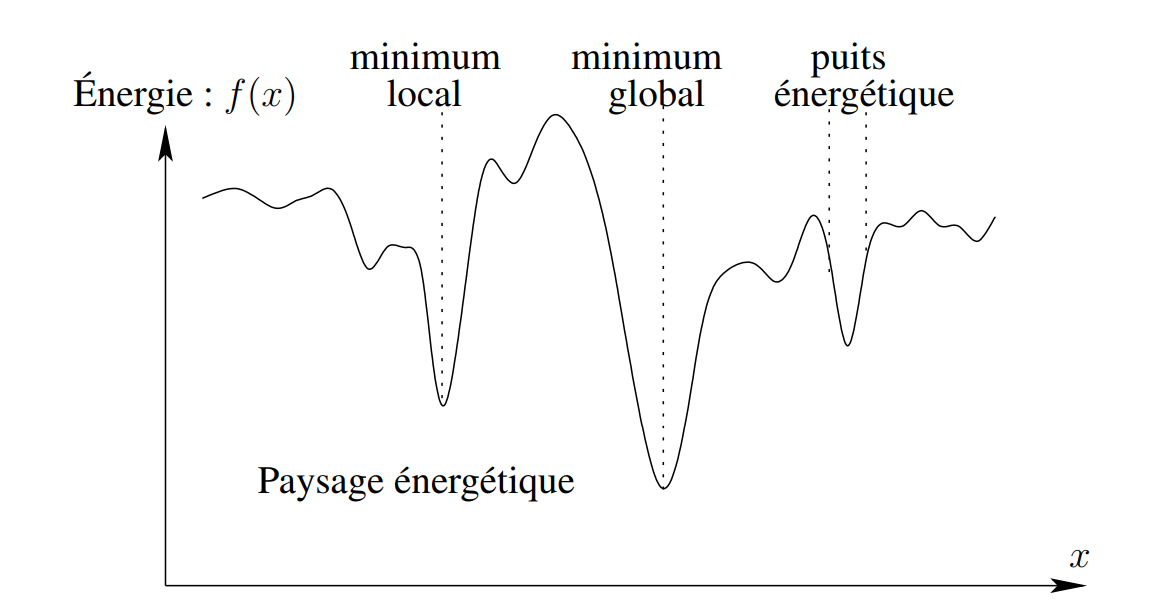
\includegraphics[height=2in]{img/Optimum_global_optimum_local.png}	
	\captionof{figure}{Paysage énergétique dans le cadre continu d’une fonction de coût pour un espace des
solutions à une dimension \citep{BICHOT2007}} \label{ogol}
\end{center}
%%%%%%%%%%%%%%%%%%%%%%%%%%%%%%%%%%%%%%%%%%%%%%%%%%%%%%%%%%%%%%%%%%%%%%%%%%%%%%%%%%%%%%%%%%%%%
%%									section.	Graphes											%
%%%%%%%%%%%%%%%%%%%%%%%%%%%%%%%%%%%%%%%%%%%%%%%%%%%%%%%%%%%%%%%%%%%%%%%%%%%%%%%%%%%%%%%%%%%%%

\section{Graphes}
Cette section rappelle quelques définitions de la théorie des graphes \citep{Francois2013}.

\begin{definition}[Graphe]
	Un graphe est un couple $G= (S, A)$, formé d'un ensemble $S$ de sommets (ou nœuds ou points) et d'un ensemble $A$ d'arêtes, d'arcs (ou lignes) qui sont associés à des sous-ensembles à deux éléments de $S$. Les sommets appartenant à une arête sont ses extrémités. Un sommet d'un graphe n'est pas nécessairement extrémité d'une arête : c'est alors un sommet isolé. La taille d'un graphe est, selon le cas, le nombre de ses sommets $\mid S \mid$ ou le nombre de ses arêtes $\mid A \mid $. Selon la nature de l'ensemble $A$, le graphe peut être orienté ou non orienté.
\end{definition}

\begin{definition}[Graphe orienté, non orienté]
	Soit un graphe $G = (S, A)$. Si $\forall (x, y) \;\in\; A$, $(y, x) \;\in\; A$, alors le graphe est dit non orienté et les éléments de $A$ sont appelés arêtes du graphe. Dans ce cas, on note indifféremment une arête : $a \;\in\; A$, $(s, s’) \;\in\; A$ avec $s$ et $s’$ dans $S$, ou encore $(s’, s)$. Dans le cas contraire, le graphe est dit orienté et les éléments de $A$ sont appelés arcs du graphe.
\end{definition}

\begin{definition}[Adjacence]
Soient un graphe $G = (S, A)$ et une arête $a = (s, s’) \;\in\; A$. On dit que les sommets $s$ et $s'$ sont les sommets adjacents (voisins) à l'arête $a$. De même, on dit que $a$ est l'arête adjacente aux sommets $s$ et $s'$.

\end{definition}

\begin{definition}[Degré d'un sommet]
Dans un graphe non orienté $G = (S, A)$, le degré d'un sommet $s \;\in\; S$ est le nombre d'arêtes auxquelles ce sommet appartient :
\begin{center}
	$deg(s) = card({(s, s') \in\; A, s' \in S})$
\end{center}
\end{definition}

\begin{definition}[Graphe Complet]
Un graphe est complet si tous ses sommets sont adjacents entre eux. Deux sommets non adjacents peuvent malgré tout avoir une certaine connections. Dans ce cas, nous parlerons de chemin.
\end{definition}

\begin{definition}[Chemin]
Un chemin dans $G = (S, A)$ de longueur $n$ est une suite de sommets $a_{1}a_{2} . . . a_{n}a_{n+1}$ reliés entre eux par des arêtes, c'est-à-dire $a_{i}a_{i+1} \;\in A$, pour $i = 1,\; 2, \; . . .,\; n$. Un cycle est un chemin fermé, C'est-à-dire que $a_{1} = a_{n+1}$.
\end{definition}

\begin{definition}[Graphe connexe]
Soit un graphe $G = (S, A)$. On dit que ce graphe est connexe si, quels que soient les sommets $s$ et $s'$ de $S$, il existe un chemin de $s$ vers $s'$. 
\end{definition}

\begin{definition}[Boucle et arête multiple]
Une arête est appelée une boucle si ses deux extrémités sont identiques. Si deux arêtes possèdent les mêmes extrémités, alors on dit que l'arête est multiple et que ces deux arêtes sont parallèles. Dans ce cas, la multiplicité d'une arête est le nombre total de ses arêtes parallèles, y compris elle-même.
\end{definition}

\begin{definition}[Graphe value ou pondéré]
Un graphe pondéré est un graphe étiqueté où chaque arêtes (arcs) est affectée d'un nombre réel positif, appelé poids de cette arête (arc).
\end{definition}

\begin{definition}[Sous-graphe]
Un sous-graphe $H = (S_H, A_H)$ d'un graphe $G = (S, A)$ est le graphe $G$ auquel des sommets et/ou des arêtes ont été enlevés, c'est-à-dire   
\begin{center}
$S_H \subseteq S$ et $A_H \subseteq A$.
\end{center}
\end{definition}

\begin{definition}[Chaîne]
	Une chaîne est une suite d'arcs partant d'un sommet $s_1$ et se terminant à un sommet $s_{n}$. Nous pouvons la définir comme suit :\begin{flushleft}
	$ G = (S, A) | S = \{s_1, s_2, ..., s_n\} \wedge A=\{a_1, a_2, ..., a_{n-1}\}\; où\; a_i = (s_i, s_i+1)\; i=1..n-1 $.
	\end{flushleft}
\end{definition}

\begin{definition}[Circuit]
Un circuit est une suite d'arcs partant et finissant au même sommet. Nous pouvons le définir comme suit: \begin{center}
$G = (S, A) | S = \{s_1, s_2, ..., s_n\} \wedge  A=\{(s_1, s_2), (s_2, s_3), ..., (s_{n-1}, s_n), (s_n, s_1)\}$
\end{center}
\end{definition}

\begin{definition}[Appariement]
Soit un graphe $G = (S, A)$. L'appariement $M$ du graphe $G$ est un ensemble d'arêtes non-adjacentes deux à deux. On dit que l'appariement est maximum lorsqu'il contient le plus grand nombre possible d'arêtes. On dit que l'appariement $M$ est maximal lorsque toute arête du graphe possède une intersection non vide avec au moins une arête de $M$.
\end{definition}

\paragraph{Remarque}
Tout appariement maximal est aussi un appariement maximum. Soit un appariement maximal $M$, si une arête quelconque de $A$ qui n'est pas dans $M$ est ajoutée à $M$, alors $M$ n'est plus un appariement de $G$. La réciproque n'est pas nécessairement exacte: soit un graphe linéaire de $4$ sommets, l'appariement composé de l'arête formée des deux sommets centraux est maximal mais pas maximum. Un graphe peut posséder plusieurs appariements maximal (et a fortiori plusieurs appariements maximum).
%%%%%%%%%%%%%%%%%%%%%%%%%%%%%%%%%%%%%%%%%%%%%%%%%%%%%%%%%%%%%%%%%%%%%%%%%%%%%%%%%%%%%%%%%%%%%
%%									section.	Theorie de jeux								%
%%%%%%%%%%%%%%%%%%%%%%%%%%%%%%%%%%%%%%%%%%%%%%%%%%%%%%%%%%%%%%%%%%%%%%%%%%%%%%%%%%%%%%%%%%%%%

\section{Théorie de jeux}

La théorie de jeux appelée aussi théorie de décision en interaction est une domaine qui inspire des mathématiques (probabilités, optimisation/contrôle, combinatoire, logique, calculabilité, complexité) et d’autre sciences tel que économie, cryptographie, physique quantique, cybernétique, biologie, sociologie, linguistique, philosophie.
Les premiers fondements de ce domaine étaient décrits autour des années 1920 par Ernst Zermelo \citep{depriester1913ernst}, Émile Borel \citep{EmileBorel1921} et John von Neumann \citep{depriester1928jonvon}. Les idées de la théorie de jeux sont ensuite développées par Oskar Morgenstern et John von Neumann en 1944 \citep{depriester1944jo}.

La théorie de jeux se propose d'étudier des situations (appelées jeux) où des individus (les joueurs) prennent des décisions, chacun étant conscient que le résultat de son propre choix (ses gains) dépend de celui des autres. Ces décisions ayant pour but un gain maximum ou un gain stabilisé.

Dans ce qui suit nous présentons les concepts qui lui sont propres.
\begin{definition}[Jeux]
Un "jeu" est une situation où des joueurs sont conduits à faire des choix stratégiques parmi un certain nombre d'actions possibles, et ce dans le cadre défini à l'avance par les "règles du jeu", le résultat de ces choix constituant une "issue du jeu", à laquelle est associé un "gain" (ou payement), positif ou négatif, pour chacun des participants.	
\end{definition}
\textbf{Remarque:} Un joueur peut être une personne, un groupe de personnes, une société, une région, un parti politique, un pays ou la Nature.

\begin{definition}[Jeux coopératif]
	Un jeu est dit coopératif lorsque les joueurs peuvent communiquer librement entre eux et passer des accords (par ex. sous forme d'un contrat). Ils forment alors une coalition et recherchent l'intérêt général suivi d'un partage des gains entre tous les joueurs.
\end{definition}
\begin{definition}[eux non coopératif]
	Un jeu non-coopératif, les joueurs (qui ne communiquent pas ou ne peuvent pas communiquer entre eux) agissent selon le principe de rationalité économique: chacun cherche à prendre les meilleures décisions pour lui-même (c'est à dire cherche à maximiser ses gains individuels).
\end{definition}

\begin{definition}[Stratégie]
	La stratégie d’un joueur est la fonction par laquelle il choisit son coup de jouer en fonction de l’état du jeu (ou de la fonction de l’état qui lui est présentée). Ainsi un jeu est constitué d'un ensemble de stratégies et de règles du jeu.  Une stratégie est dite gagnante lorsque le joueur qui l’utilise gagne le jeu (supposé avoir une notion de « joueur gagnant ») quels que soient les coups choisis par l’autre joueur.	
\end{definition}

\begin{definition}[Stratégie pure]
	Une stratégie pure du joueur $J_i$ est un plan d’action qui prescrit une action de ce joueur pour chaque fois qu’il est susceptible de jouer. L’ensemble des stratégies pures du joueur $J_i$ est noté par $S_i$.
\end{definition}

\begin{definition}[Stratégie mixte]
	Une stratégie mixte du joueur $J_i$ est une distribution de probabilités $p_i$ définie sur l’ensemble des stratégies pures du joueur $J_i$. L’ensemble des stratégies mixtes du joueur $J_i$  est noté note $\sum_i$.
\end{definition}

\begin{definition}[Stratégie locale]
	Une stratégie locale du joueur $J_i$ est un ensemble d’information $A$ et une distribution de probabilités sur l’ensemble des actions disponibles en cet ensemble d’information. L’ensemble des stratégies locales du joueur $J_i$ pour l’ensemble d’information $A$  est $\pi_{iA}$.
\end{definition}

\begin{definition}[Stratégie comportementale]
	Une stratégie comportementale du joueur $J_i$ est un vecteur de stratégies locales de ce joueur, contenant une stratégie locale par ensemble d’information de ce joueur. On note $\pi_i$ l’ensemble des stratégies comportementales du joueur $J_i$.
\end{definition}

\begin{definition}[Jeux sous forme stratégique]
	Un jeu sous forme stratégique est défini par:
	\begin{itemize}
		\item Un ensemble $N = \{1, . . ., n\}$ de joueurs.
		\item Pour chaque joueur $J_i$ un ensemble de stratégies $ S_i = \{s_1, . . ., s_n\}$.
		\item Pour chaque joueur  $J_i$ une fonction dévaluation $\mu_i$: $s_1 \times . . . \times s_n \longrightarrow IR$, qui à chaque ensemble de stratégies associe les gains du joueur $J_i$.
	\end{itemize}
\end{definition}

\begin{definition}[Profil stratégique]
	Un profil stratégique $(s_1*, …, s_n*)$ est une solution d’un jeu, on peut justifier que des joueurs rationnels, guidés par leur intérêt personnel, le jouerait.
\end{definition}

\begin{definition}[Stratégie dominante]
	Un stratégie $s_i*$ d’un joueur est une stratégie dominante lorsque pour tout profil de stratégies des autres joueurs, le gain du joueur est maximum lorsqu’il joue cette stratégie.
\end{definition}

\begin{definition}[Équilibre]
	On dit qu’un jeu possède un équilibre en stratégies dominantes s’il admet un profil stratégique composé uniquement de stratégies dominantes des joueurs.
\end{definition}

\begin{definition}[Équilibre de Nash]
On dit qu’un jeu possède un équilibre de Nash s’il admet un profil stratégique $(s_1*, …,s_n*)$, tel que chaque stratégie individuelle de ce profil est une meilleure réponse aux stratégies des autres joueurs.
\end{definition}
%%%%%%%%%%%%%%%%%%%%%%%%%%%%%%%%%%%%%%%%%%%%%%%%%%%%%%%%%%%%%%%%%%%%%%%%%%%%%%%%%%%%%%%%%%%%%
%%									section.	Partitionnement de graphe											%
%%%%%%%%%%%%%%%%%%%%%%%%%%%%%%%%%%%%%%%%%%%%%%%%%%%%%%%%%%%%%%%%%%%%%%%%%%%%%%%%%%%%%%%%%%%%%

\section{Partitionnement de graphe}
Le partitionnement de graphe est un problème NP-Complet \citep{GAREY1976}, utilisé pour résoudre un grand nombre de problèmes d'ingénierie : La conception de circuits intégrés électroniques \citep{CONG2003}, la répartition de charge pour les machines parallèles \citep{BARAT2016}, la dynamique des fluides, le calcul matriciel, la segmentation d'images \citep{GRADY2006} ou la classification d'objets \citep{DHILLON2007}.

Etant donné un graphe non-orienté $G = (S, A)$ où $S$ est l'ensemble des sommets et $A$ est l'ensemble des arêtes. Les sommets et les arêtes peuvent être pondérés. Le problème du partitionnement d'un graphe $G$ consiste à le diviser en $k$ parties disjointes. Du point de vue mathématique, on peut partitionner les sommets ou bien les arêtes. Cependant, bien que certains problèmes cherchent à partitionner les arêtes d'un graphe \citep{HOLYER1981}, on entend le plus souvent par partition d'un graphe, le partitionnement des sommets de ce graphe.

\begin{definition}[Partition des sommets d'un graphe] \citep{BichotSiarry2013}
\\Soient un graphe $G = (S,A)$ et un ensemble de $k$ sous-ensembles de $S$, noté $P_k = \{S_1, S_2, . . . ,S_n\}$. En d'autres termes, $P_k$ est dite une partition de $G$ si :
\begin{itemize}
	\item Aucun sous-ensemble de $A$ qui est élément de $P_k$ n'est vide : $\forall i\; \in \; \{1, ..., k\},\; S_i \ne \emptyset$
	\item Les sous-ensembles de $S$ qui sont éléments de $P_k$ sont disjoins deux à deux : $\forall(i, j) \in{1, ..., K}, i \ne j, S_i \cap S_j = \emptyset$
	\item L'union de tous les éléments de $P_k$  est $S$ : $U^{k}_{i=1} S_k = S$
\end{itemize}
Les éléments $S_i$ de $P_k$ sont appelés les parties de la partition.\\
Le nombre $k$ est appelé le cardinal de la partition, ou encore le nombre de parties de la partition.
Dans le cas $k = 2$, on a le problème de bissection.
\end{definition}
%%%%%%%%%%%%%%%%%%%%%%%%%%%%%%%%%%%%%%%%%%%%%%%%%%%%%%%%%%%%%%%%%%%%%%%%%%%%%%%%%%%%%%%%%%%%%
%%									section.	Approches de partitionnement										%
%%%%%%%%%%%%%%%%%%%%%%%%%%%%%%%%%%%%%%%%%%%%%%%%%%%%%%%%%%%%%%%%%%%%%%%%%%%%%%%%%%%%%%%%%%%%%

\section{Approches de partitionnement de graphes}
 Le partitionnement d'un graphe consiste à trouver une partition des sommets respectant une ou plusieurs propriétés. Ces propriétés sont de nature très diverses. On peut par exemple chercher à minimiser la capacité des arêtes externes, c'est-à-dire le nombre d'arêtes ou la somme totale des poids des arêtes reliant deux groupes.  Le problème devient difficile si on cherche à diviser le graphe en $k$ groupes de tailles équilibrées car il n'existe alors pas d'algorithme polynomial pour y répondre. Ce problème a été démontré NP-complet \citep{HYAFIL1973}, \citep{GAREY1976}

Au cours des dernières années, beaucoup d'efforts ont été consacrés au développement d'heuristiques rapides et efficaces pour ce problème. Ces heuristiques peuvent souvent gérer des graphes assez grands avec des milliers de nœuds et fournir de bonnes solutions. Pour un aperçu plus détaillé, nous nous référons à \citep{BichotSiarry2013}, \citep{BULU2016},\citep{SCHLOEGEL2000}.

Nous allons maintenant présenter les approches couramment utilisées pour résoudre le problème du partitionnement de graphes.


\subsection*{Approche exacte}
Les solutions exactes peuvent être utilisées comme des facteurs importants pour valider les heuristiques. Cependant, peux d'effort ont été faits dans le développement d'algorithmes exacts \citep{Armbruster2008}, \citep{Bonami2012}, \citep{Delling2012}, \citep{FeldmannWidmayer2015}, \citep{Ferreira1998}, \citep{Hager2013}, \citep{Kaibel2011}, \citep{Sellmann2003}, \citep{Sorensen2007}. La plupart de ces méthodes reposent sur la méthode de séparation et d'évaluation qui permet d'éviter l'exploration systématique de l'espace des solutions en éliminant les sous-arbres menant à des solutions moins bonnes qu'une solution donnée, et se diffèrent selon que l'exploration de l'arbre est réalisée en profondeur, par niveaux ou par ordre croissant des valeurs des fils non encore traités \citep{Land2010}.
Du fait de la nature NP-difficile du problème, il est clair que généralement seuls des graphes relativement petits peuvent être résolus par une approche exacte.

\subsection*{Approche spectrale}
L'approche spectrale du partitionnement de graphes repose sur le théorème spectral de l'algèbre linéaire, elle consiste à rechercher les valeurs propres de la matrice de Laplace associée au graphe $G$, ensuite l'ordonnancement de ces valeurs qui est lié à la connectivité des sommets du graphe.
Les techniques spectrales ont d'abord été utilisées par Donath et Hoffman \citep{DonathHoffman1972} et Fiedler \citep{Fiedler1973}, \citep{Fiedler1975}, et ont été améliorées par la suite par plusieurs chercheurs \citep{Boppana1987}, \citep{HendricksonLeland1995a}, \citep{Kabelikova2006}, \citep{Simon1991}.
Il a été montré que cette méthode permet d'obtenir un extremum global avec certains graphes \citep{Pothen1990}; cependant, il a aussi été mis en évidence que cette méthode est très coûteuse en terme de calculs et devient inefficaces lorsque la taille du graphe devient importante \citep{BarnardSimon1994}.

\subsection*{L'approche combinatoire} \citep{BENSETIRA2017}
Contrairement à l'approche spectrale, les travaux cités dans cette approche opèrent directement sur la structure du graphe.
L'idée générale consiste à effectuer un parcours de proche en proche d'une partie de l'ensemble $P(G)$ afin d'y trouver le meilleur candidat qui résolve le problème. En plus, un algorithme de ce type nécessite les deux données suivantes :
\begin{itemize}
\item la définition d'un voisinage dans $P(G)$;
\item l'historique des optimisations précédentes.
\end{itemize}
Le voisinage permet de définir comment l'algorithme va progresser en perturbant la solution courante $S$ : par exemple, on peut définir le voisinage de $S$ comme correspondant à un seul déplacement de sommet par l'ensemble des éléments de $P(G)$ qui peuvent être obtenus en changeant dans la partie un seul sommet de $S$.

Dans cette approche, on distingue entre les méthodes basées sur les algorithmes itératifs et les méthodes basées sur les méta-heuristiques.

\subsection*{Les algorithmes itératifs}
Les algorithmes itératifs d'optimisation fonctionnent en partant d'une partition $\prod _0 \;\in \; P(G)$ de $G$, valide et bien équilibrée, et se déplacent dans l'espace des solutions en sélectionnant le voisin le plus proche qui permet de réduire la coupe de la partition. L'algorithme s'arrête lorsqu'aucun des voisins n'est satisfaisant. Ces algorithmes convergent donc vers l'optimum local accessible depuis la partition initiale $\prod _0$ .

Bien que la convergence ne soit que locale et dépendante du point de départ dans $P(G)$, ces algorithmes sont très populaires. Les résultats produits pouvant être améliorés en effectuant plusieurs exécutions à partir de partitions initiales différentes ou en utilisant le schéma multi-niveaux qui sera présenté plus loin. Parmi les algorithmes de cette catégorie, nous pouvons citer \citep{FiducciaMattheyses1988}, \citep{Hagen1997}, \citep{KernighanLin1970}, \citep{Krishnamurthy1984}. 

Le principal défaut de ces approches itératives concerne leur vision strictement locale du problème, ce qui implique que le résultat ne peut être au mieux qu'un optimum local, fortement dépendant de la solution initiale. D'autres approches d'algorithmes d'optimisation ayant une vision plus globale peuvent être utilisées.

\subsection*{Les approches basées sur les méta-heuristiques}
 Les algorithmes génétiques, ont fait l'objet de plusieurs approches pour le problème du partitionnement de graphes \citep{BuiMoon1996}, \citep{ChevalierPellegrini2006}, \citep{ChockalingamArunkumar1992}, \citep{Soper2004}, \citep{TalbiBessiere1991}.  Le principe est d'explorer l’espace des solutions à l'aide d'une population d'individus qui vont échanger entre eux certaines de leurs caractéristiques lors d'une étape de reproduction, ceci dans le but d'obtenir de nouveaux individus combinant les qualités de leurs parents tout en essayant d'en diminuer les défauts. Pour un aperçu général des algorithmes génétiques abordant le problème du partitionnement de graphe, nous renvoyons le lecteur à l'article de \citep{Kim2011}.

Les principales difficultés d'application de ces algorithmes tiennent d'une part à la multitude de paramètres qu'il faut régler en fonction de la nature du problème, d'autre part à leurs coûts en mémoire et en temps : La taille de la population est liée à celle du problème et le temps est dépendant du nombre de générations qui est lié à la taille de la population.

Les méthodes de colonies de fourmis consistent à imiter le comportement des fourmis qui exploitent une méthode de résolution collective. En effet, les fourmis utilisent des phéromones pour marquer les différents chemins empruntés et la concentration de ces marqueurs chimiques est
d'autant plus importante que la fréquence d'utilisation est importante. Pour le k-partitionnement, l'idée est donc d'utiliser $k$ colonies de fourmis dont le but est d'accumuler la nourriture qui est distribuée sur les sommets du graphe, l'exploration est guidée par la répartition des colonies, de la nourriture et par les décisions des fourmis \citep{Korosec2004}, \citep{LanghamGrant1999}, \citep{Jovanovic2016}.

D'autres méta-heuristiques, comme la recherche tabou \citep{BattitiBertossi1999}, le recuit simulé \citep{Bichot2004}, \citep{Johnson1989}, \citep{Williams1991}, les algorithmes de gradients aléatoires adaptatifs (GRASP) \citep{AreibiYang2004}, les méthodes de diffusion stochastique \citep{TaoZhao1993}, \citep{Wan2005}, ont été appliquées avec plus ou moins de succès au partitionnement de graphe.

On peut aussi citer les travaux basés sur la méthode de percolation \citep{MeyerhenkeSchamberger2006}, \citep{Pellegrini2007} qui s'inspire du principe de l'écoulement d'un fluide à travers un solide poreux, et la méthode de fusion-fission \citep{Bichot2007} qui s'inspire de la physique nucléaire et plus particulièrement des fusions et fissions d'atomes.
L'efficacité des méthodes combinatoires est étroitement liée à la taille de l'espace de recherche, les heuristiques calculent un partitionnement acceptable en un temps polynomial.


\subsection*{L'approche multi-niveaux}
La méthode multi-niveaux, introduite par \citep{BarnardSimon1994}, \citep{HendricksonLeland1995b}, \citep{VanDriesscheRoose1994}, permet de réduire la taille du graphe ainsi que celle de l'espace de recherche tout en procurant l'accès à une vision globale pour les algorithmes
combinatoires. L'idée principale est de travailler sur un graphe réduit ayant les mêmes propriétés topologiques que le graphe initial (regrouper les sommets ensemble pour traiter de groupes de sommets plutôt que de sommets indépendants).
Pour ce faire, le schéma multi-niveaux comporte trois étapes (Figure \ref{pmn}) :
\begin{enumerate}
	\item  L'étape de contraction, durant laquelle on applique récursivement une fonction de contraction afin de diminuer la taille du graphe;
	\item  L'étape de partitionnement initial, où l'on applique une heuristique sur le plus petit graphe;
	\item  L'étape d'affinage, durant laquelle la partition initiale est projetée et raffinée sur les graphes de plus en plus gros jusqu'au graphe initial.
\end{enumerate}
  
	\begin{center}
		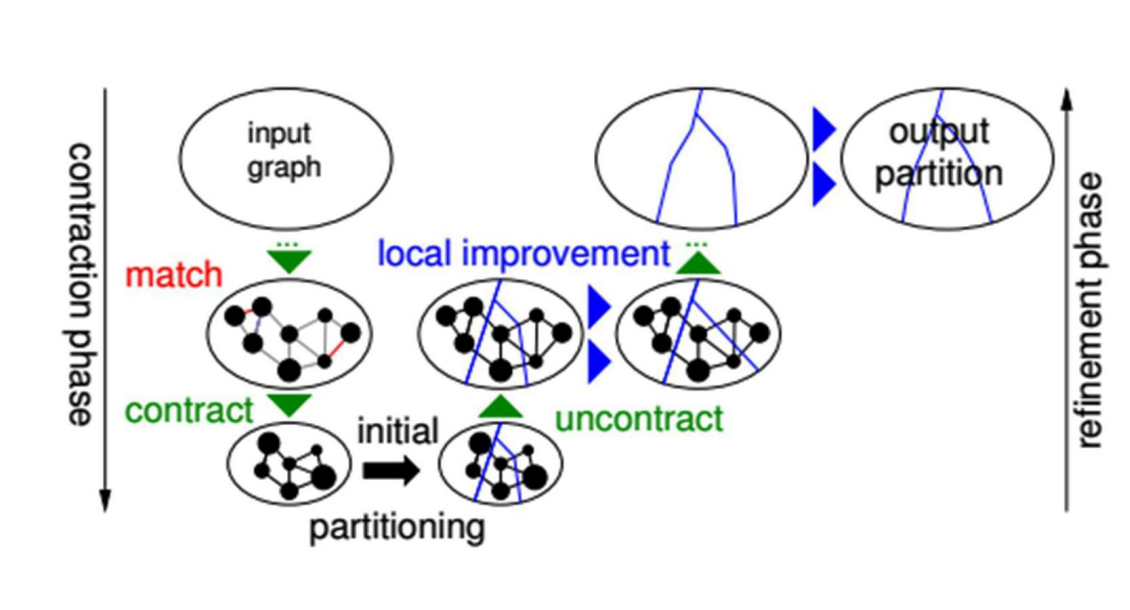
\includegraphics[height=2in]{img/multiniveaupartitionnement.PNG}		
		\captionof{figure}{ L'approche multi-niveau du partitionnement de graphe, \citep{SandersSchulz2011}} \label{pmn}
	\end{center}
Dés lors, plusieurs améliorations ont été proposées \citep{Aurora2007}, \citep{ChevalierSafro2009}, \citep{KalayciBattiti2018}, \citep{Karypis2003}, \citep{KarypisKumar1998}, \citep{Monien2000}, \citep{Pellegrini1995}, \citep{Pope2016}, \citep{Predari2017}, \citep{Safro2015}, \citep{SandersSchulz2011}, \citep{Talu2017}.


\subsection*{La parallélisation du partitionnement de graphes}
Des tentatives de parallélisation des algorithmes de partitionnement de graphes ont vu le jour. On peut citer ParMeTiS \citep{Karypis2011}, ParJostle \citep{Walshaw2012}, PT-Scotch \citep{ChevalierPellegrini2008}, et Parkway \citep{TrifunovicKnottenbelt2004} pour le partitionnement d'hyper-graphes. Tous ces outils utilisent un schéma multi-niveaux parallèle.

Des approches qui combinent les différentes méthodes présentées ci dessus ont été proposées, \citep{Chan2016}, \citep{LaSalleKarypis2013}, \citep{LaSalleKarypis2015}, \citep{LengYu2007}, \citep{Rahimian2013}, \citep{SandersSchulz2012}, \citep{Tashkova2011}.



%%%%%%%%%%%%%%%%%%%%%%%%%%%%%%%%%%%%%%%%%%%%%%%%%%%%%%%%%%%%%%%%%%%%%%%%%%%%%%%%%%%%%%%%%%%%%
%%									section.	Distribution de graphes											%
%%%%%%%%%%%%%%%%%%%%%%%%%%%%%%%%%%%%%%%%%%%%%%%%%%%%%%%%%%%%%%%%%%%%%%%%%%%%%%%%%%%%%%%%%%%%%

\section{Distribution de graphes}
Le contexte général de notre projet de fin d'étude est la vérification formelle des systèmes. Les systèmes à vérifier sont représentés par des modèles de spécification formels, qui génèrent sous une sémantique formelle des espaces d'états. Un espace d'états peut être considéré comme un graphe. Dans ce contexte particulier, on parle de distribution de graphes (espaces d'états), et non pas de partitionnement de graphe. Les différences principales entre eux résident dans le fait que:
\begin{itemize}
\item  Le partitionnement des graphes opèrent sur des graphes simples non orientés et pondérés. Alors que dans notre contexte, les graphes sont orientés, non pondérés, et contiennent dans la plupart des cas des cycles.
\item  En générale, les applications qui utilisent le partitionnement des graphes supposent l'existence préalable du graphe. Tandis que les espaces des états sont construits au moment de leurs distribution.
\item La distribution d'un graphe n'interdit pas la duplication de certains de ses états (sommets) sur plusieurs parties distribuées du graphes.
\end{itemize}

\subsection*{L'espace d'états distribué}{
Dans cette section, nous définissons la structure d'un espace d'états distribué qui se compose de sous-graphes localisés dans les différentes machines disponibles sur le réseau. 


Un espace d'état est une structure relationnelle qui représente le comportement d'un système (programme, protocole, réseau social, ...). Il représente tous les états possibles du système et les transitions entre eux. Un espace d'états est un graphe orienté $G = (S, A)$ avec un ensemble de sommets $S$, un ensemble d'arcs $A$.}


\begin{definition}
Soit $M =\{M_K\}_{K=1..N}$ $N$ machines. Un espace d'états distribué, noté $DiG$, est un graphe avec une fonction de distribution $f^k$. $DiG = (G; f^k )_{ k=1..N}$ , tel que : $G = (S, A)$ : est un graphe dirigé.
$f^k : G \Rightarrow G_k$ : est une application de G dans G k , tel que \\$G_k = (S_k , A_k )$ : $\{G_K \}_{1<k<N}$ est un ensemble de sous-ensembles appelés fragments $G_k $, tel que :\\ $U^{N}_{k=1} S_k = S\; et\; U^{N}_{k=1}A_k = A$
\end{definition}

\begin{definition} \citep{BENSETIRA2017}\\
Un fragment $G_k$ est définit par $G_k = (S_k , A_k )$ de tel sorte que :
\begin{itemize}
\item $S_k\subseteq S$ est un fragment des états de $S$ dans la machine $M_k$ tel que :
	\begin{itemize}
	\item  Aucun élément de $S_k$ n'est vide : $\forall \;k \in \;1, ..., N,\; S_k \ne \emptyset$
	\item L'union de tous les éléments de $S_k$ est égale à $S$ : $U^{N}_ {k=1} S_k = S$
	\end{itemize}
\item $A_k = A^{L}_{K}\cap A^{K}_{R}$ tel que  $A^{L}_{K} \cap A^{K}_{R}= \emptyset$ : l'ensemble des transitions internes et externes avec :
	\begin{itemize}
	\item  $A^{L}_{K}\subseteq S_K \times S_K$ est l'ensemble des transitions entre les états qui appartient à la même machine $M_k$ (transitions locales ou internes)
	\item  $A^{R}_{K}\subseteq S_K \times (S/S_K ) \cup (S/S_K ) \times S_K = (s, s')$, tel que soit $(s \in S_K et s' \neq S_K ) ou(s \neq S_K et s'
\in S_K )$ : est l'ensemble des transitions dont les origines se trouvent dans des machines locales et les états cibles (destination) sont dans des machines distantes (transitions externes) et inversement.
	\end{itemize}
	
\end{itemize}
Le nombre $k$ est appelé la cardinalité du fragment.
\end{definition}

La Figure \ref{eed}(a) représente un espace d'états, et une distribution possible de cet espace sur un réseau de trois machines (Figure \ref{eed}(b)). Les transitions internes sont marquées avec des lignes continues, et les transitions externes sont marquées avec des lignes en pointillés.

\begin{center}
		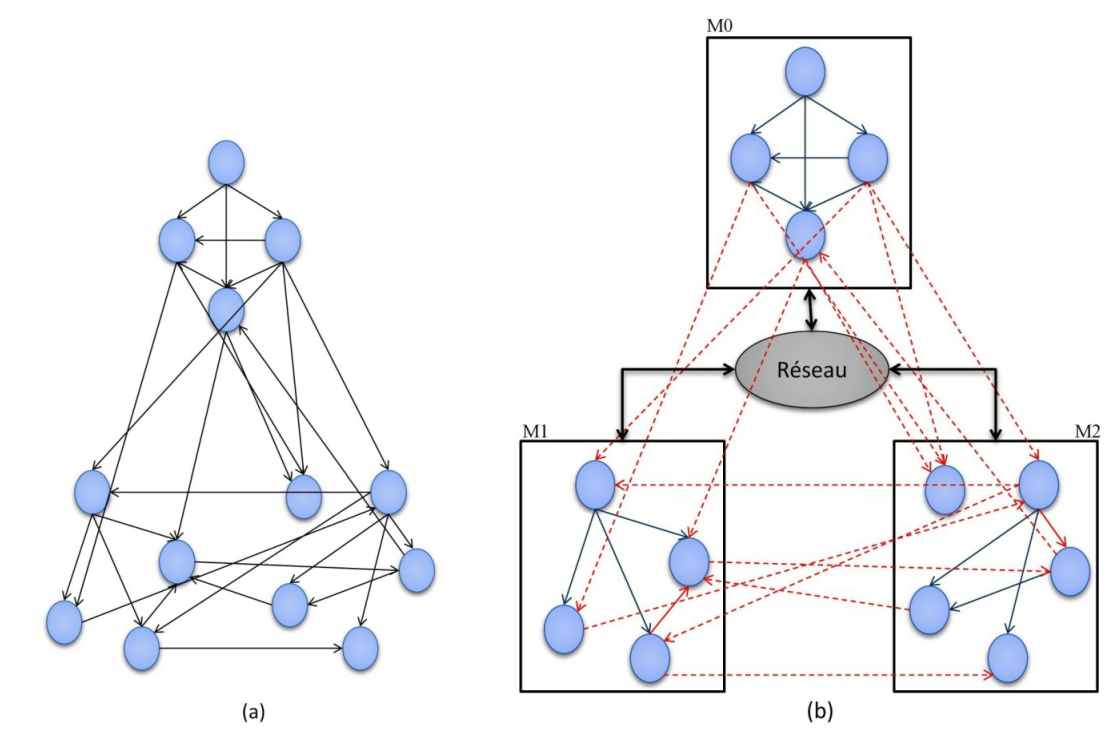
\includegraphics[height=3in]{img/eed.PNG}		
		\captionof{figure}{Un espace d’état et sa distribution sur un cluster de 3 machines, \citep{BENSETIRA2017}} \label{eed}
\end{center}

\subsection*{Approche de distribution des espaces d'états}
\paragraph{Distribution basée sur des fonctions}
 La plupart des solutions proposées pour la distribution des espaces d'états reposent sur l'utilisation d'une fonction de distribution qu'elle soit statique \citep{Garavel2013}ou dynamique \citep{Allmaier1997}, basée sur la structure de formalisme de spécification utilisé \citep{Ciardo1998}, \citep{BlomOrzan2005} ou guidée par des heuristiques \citep{Rodrigues2006}.
 \paragraph{Distribution basée sur la coloration}
 Cette approche consiste à introduire le concept de coloration et la relation de dominance dans les graphes pour trouver la bonne distribution des graphes L'approche proposée dans \citep{Guidoum2013} est basée sur le concept de la coloration forte stricte des graphes \citep{Bouzenada2012}. L'approche proposée est divisée en deux parties : un processus d'initialisation et un processus d'optimisation. Dans la première étape, les auteurs utilisent l'algorithme de coloration \citep{Bouzenada2012} qui assure la propriété de dominance. Les sorties de ce dernier (le nombre de couleurs dominées, ensemble de sommets colorés) sont exploitées pour répartir initialement le graphe et obtenir des parties disjointes. Ensuite le processus d'optimisation est utilisé pour trouver la bonne distribution.
 
 \paragraph{Distribution basé sur les métaheuristiques}
Récemment une nouvelle alternative de distribution des espaces d'états a été investiguée. Les approches proposées dans cette classe se basent sur l'utilisation des méthodes d'optimisation combinatoire, qui ont montré leur efficacité de résolution des problèmes dans différents domaines d'application.
 \\\\ 
Saidouni et al. \citep{Saidouni2012} proposent un nouvel algorithme de distribution inspiré de l'algorithme d'optimisation par essaims de particules. Les auteurs ont pu montrer comment les composants de la métaheuristique PSO comme le voisinage, les particules, et leurs vitesses et direction peuvent être adaptés pour la distribution des graphes sur une plateforme de N machines. L'approche fournit un bon équilibrage de charge et une réduction des connexions externes dans le réseau. Cependant, cette approche souffre du problème des états redondants.
\\\\
Une autre approche a été développée dans  \citep{TabibSaidouni2016},  \citep{Tabib2017}, où les auteurs ont proposé un algorithme génétique basé sur la loi gravitationnelle de Newton pour la distribution de graphes. La particularité de cette approche est que les espaces d'états sont codés par les diagrammes de décision binaires, et l'utilisation d'un modèle génétique en ilot qui repose sur l'exécution parallèle de plusieurs machines qui contiennent des populations de même taille avec la migration de leur m meilleurs individus chaque $n$ cycles.
\\\\
Saidouni et Bensetira \citep{BENSETIRA2017}, proposent un nouvel algorithme de distribution de l'espace d'états basée sur le comportement des systèmes. La particularité de cette approche est que les états sont analysés, ensuite, selon les informations pertinentes sur les états et leurs connexions (transitions internes et externes), ils sont redistribués selon une certaines heuristiques afin d'optimiser les performances
du système. Cela se fait en définissant une bonne localité d'un état comme celle qui optimise à la fois l'équilibre de la charge de travail et la quantité de communication entre les machines engendrés par l'exécution de l'application opérant sur l'espace d'états distribués.
\section{Conclusion}{
Dans ce chapitre, nous avons introduit quelques notions sur les graphes, ensuite nous avons donné un bref aperçu du travail qui a été fait sur le partitionnement et la distribution des graphes. Il nous est alors possible de développer de nouveaux algorithmes de distribution de graphe en exploitant le model cheching et les méthodes  d'optimisation combinatoire.
}